\begin{enumerate}[label=\thesubsection.\arabic*,ref=\thesubsection.\theenumi]


\item Find the values of $k$ for which the line 
\begin{align}
(k-3)x-(4-k^2)y+k^2-7k+6=0 \label{eq:chapters/11/10/4/1/1}
\end{align}
is
\begin{enumerate}
\item Parallel to the $x$-axis
\item Parallel to the $y$-axis
\item Passing through the origin
\end{enumerate}
    \solution 
		The parameters of the given line are
\begin{align}
\vec{n}^{\top}\vec{x}=c \label{eq:chapters/11/10/4/1/2}
\end{align}
This equation can be expressed in the form of 
\begin{align}
\vec{n} = \myvec{k-3\\-4+k^2}, c  = -k^2+7k-6
\end{align}
\iffalse
Then \eqref{eq:chapters/11/10/4/1/1} can be expressed as
\begin{align}
\myvec{k-3 & -4+k^2}\vec{x} &=-k^2+7k-6\label{eq:chapters/11/10/4/1/4}
\end{align}
\fi
\begin{enumerate}
%part-1
    \item 
	    In this case,
	    \iffalse
The normal vector of $x$-axis is given by
\begin{align}
\myvec{0\\1}
\end{align}
\fi
equating $\vec{n}$ to the normal vector of $x$-axis,
\begin{align}
\myvec{k-3\\-4+k^2} &=\alpha\myvec{0\\1}\label{eq:chapters/11/10/4/1/6}
\\
\implies
k &=3
\end{align}
Substituting the value of $k$ in \eqref{eq:chapters/11/10/4/1/1}, the desired equation is
\begin{align}
        \myvec{0 & 5}\vec{x} &=6
\end{align}

\item In this case, 
equating $\vec{n}$ to the normal vector of $y$-axis,
\begin{align}
\myvec{k-3\\-4+k^2} &=\beta\myvec{1\\0}\label{eq:chapters/11/10/4/1/11}
\\
	\implies k &=\pm2
\end{align}
Substituting the value of $k$ in \eqref{eq:chapters/11/10/4/1/1}, the desired equation is 
\begin{align}
        \myvec{-1 & 0}\vec{x} &=4, \quad  k &=2\\
        \myvec{-5 & 0}\vec{x} &=-24, \quad  k &=-2
\end{align}
\item 
	In this case, 
\begin{align}
	c = 0 \implies 
	-k^2+7k-6 &= 0\\
	\implies k =1 \text{ or } k&=6
\end{align}
Substituting the value of $k$ in \eqref{eq:chapters/11/10/4/1/1}, the desired equations are 
\begin{align}
        \myvec{-2 & -3}\vec{x} &=0, \quad  k &=1\\
       \myvec{3 & 32}\vec{x} &=0, \quad  k &=6
\end{align}
\end{enumerate}

	\item Find the  equations of the lines, which cutoff intercepts on the axes  whose sum and product are 1 and -6 respectively.
\\
\solution
		Let the intercepts be $a$ and  $b$. Then
\begin{align}
a+b=1,
ab=-6 \label{eq:11/10/4/32a}
\\
\implies  a = 3, b = -2
\end{align}
Thus, the possible 
intercepts are
\begin{align}
\myvec{3\\0}, \myvec{0\\-2},
\myvec{-2\\0}, \myvec{0\\3}
\end{align}
From
		\eqref{prop:lin-eq-unit-mat},
\begin{align}
	\myvec{3 & 0 \\ 0 &-2}\vec{n} = \myvec{1 \\ 1}
	\\
	\implies \vec{n} = \myvec{\frac{1}{3} \\ -\frac{1}{2}}
	\\
	\text{or, } \myvec{2 & -3}\vec{x} = 6
\end{align}
using		\eqref{prop:lin-eq-unit}.
Similarly, the other line can be obtained
as
\begin{align}
	\myvec { 3 & -2 }  \vec{x}  = -6        
\end{align}
See  
\figref{fig:11/10/4/3line segmenta}.
\begin{figure}[!htbp]
\centering
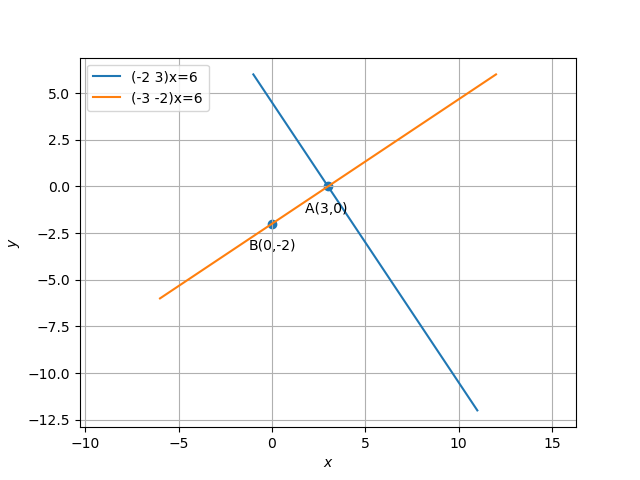
\includegraphics[width=\columnwidth]{chapters/11/10/4/3/figs/inter.png}
\caption{}
\label{fig:11/10/4/3line segmenta}
\end{figure}

\item A ray of light passing through the point $\vec{P} = \brak{1, 2}$ reflects on the x-axis at point $\vec{A}$ and the reflected ray passes through the point $\vec{Q} =\brak{5, 3}$. Find the coordinates of $\vec{A}$.
\\
    \solution 
			From \eqref{eq:11/10/4/22},
the reflection of $\vec{Q}$ is 
\begin{align}
\vec{R}  
= \myvec{5\\-3}
\end{align}
Letting
\begin{align}
\vec{A} = \myvec{x\\0},
\end{align}
since 
$\vec{P},
\vec{A},  
\vec{R}  
$
are collinear, 
		from \eqref{prop:lin-dep-rank},
\begin{align}
	\myvec{
		1 & 1 & 2 
		\\ 
		1 & 5 & -3 
		\\
		1 & x & 0 }
	\xleftrightarrow[R_3=R_3 - R_1]{R_2 = R_2 - R_1}
	\myvec{
		1 & 1 & 2 
		\\ 
		0 & 4 & -5 
		\\
		0 & x-1 & -2 }
	\\
	\xleftrightarrow[]{R_3 = 4R_3 - \brak{x-1}R_2}
	\myvec{
		1 & 1 & 2 
		\\ 
		0 & 4 & -5 
		\\
		0 & 0 & 5x-13 }
	\implies x = \frac{13}{5}
\end{align}
See  
\figref{fig:chapters/11/10/4/22/1}.
\begin{figure}[H]
\centering
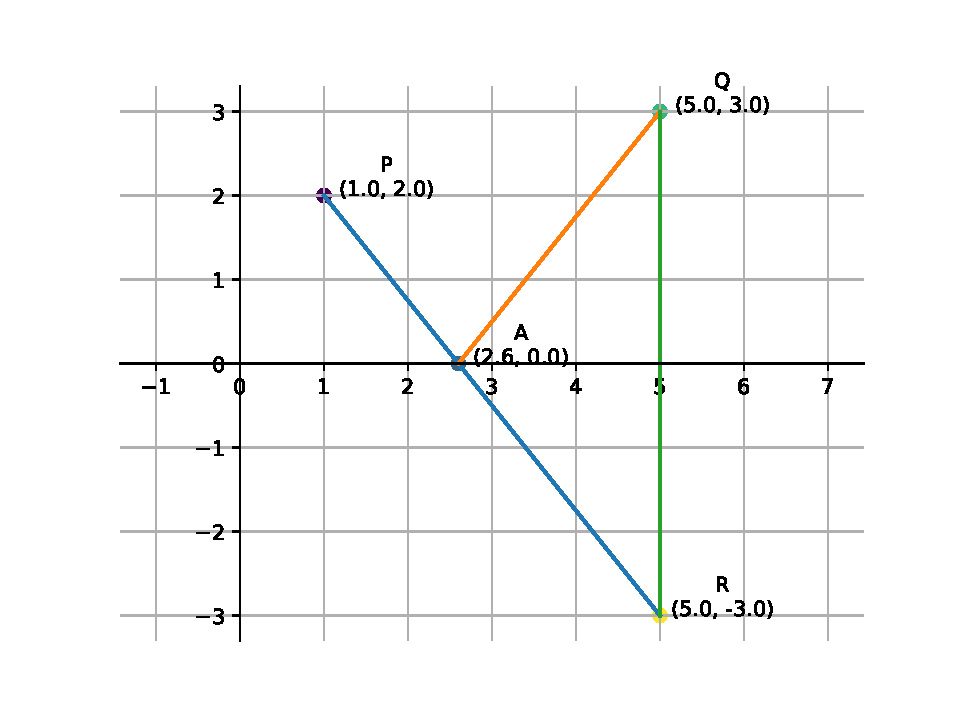
\includegraphics[width=0.75\columnwidth]{chapters/11/10/4/22/figs/fig.pdf}
\caption{}
\label{fig:chapters/11/10/4/22/1}
\end{figure}




\item Prove that in any $\triangle{ABC}$, cos A=$\frac{b^2+c^2-a^2}{2bc}$, where a,b,c are the magnitudes of the sides opposite to the vertices A,B,C respectively.
\item Distance of the point $(\alpha, \beta, \gamma)$ from y-axis is
\begin{enumerate}
	\item $\beta$ 
	\item $\abs{\beta}$
	\item $\abs{\beta+\gamma}$
	\item $\sqrt{\alpha^2+\gamma^2}$
\end{enumerate}
\item The reflection of the point $(\alpha, \beta, \gamma )$ in the xy-plane is 
\begin{enumerate}
	\item $\alpha,\beta,0)$
	\item $(0,0,\gamma)$
	\item $(-\alpha,-\beta,\gamma)$
	\item $(\alpha,\beta,-\gamma)$
\end{enumerate}
\item The plane $ax+by=0$ is rotated about its line of intersection with the plane $z=0$ through an angle $\alpha.$ Prove that the equation of the plane in its new position is 
\begin{align*}
	ax+by \pm (\sqrt{a^2+b^2} \tan\alpha)z=0.
\end{align*}
\item The locus represented by $xy+yz=0$ is 
\begin{enumerate}
	\item A pair of perpendicular lines
	\item A pair of parallel lines
	\item A pair of parallel planes 
	\item A pair of perpendicular planes
\end{enumerate}
\item For what values of $a$ and $b$ the intercepts cut off on the coordinate axes by the line $ax+by+8=0$ are equal in length but opposite in signs to those cut off by the line $2x-3y=0$ on the axes.
\item If the equation of the base of an equilateral triangle is $x+y=2$ and the vertex is (2,-1), then find the length of the side of the triangle. 
\item A variable line passes through a fixed point $\vec{P}$. The algebraic sum of the perpendiculars drawn from the points (2,0), (0,2) and (1,1) on the line is zero. Find the coordinates of the point $\vec{P}$.  
\item A straight line moves so that the sum of the reciprocals of its intercepts made on axes is constant. Show that the line passes through a fixed point. 
\item If the sum of the distances of a moving point in a plane from the axes is $l$, then finds the locus of the point.  
\item $\vec{P}_1,\vec{P}_2$ are points on either of the two lines $y-\sqrt{3}\abs{x}=2$ at a distance of 5 units from their point of intersection. Find the coordinates of the root of perpendiculars drawn from $P_1, P_2$ on the bisector of the angle between the given lines.
\item If $p$ is the length of perpendicular from the origin on the lien $\frac{x}{a}+\frac{y}{b}=1$ and $a^2,p^2,b^2$ are in A.P, then show that $a^4+b^4=0$.
\item The point (4,1) undergoes the following two successive transformations :
\begin{enumerate}
\item Reflection about the line $y=x$
\item Translation through a distance 2 units along the positive $x$-axis 
\end{enumerate}
Then the final coordinates of the point are
\begin{enumerate}
\item (4,3)
\item (3,4)
\item (1,4)
\item $\frac{7}{2}$,$\frac{7}{2}$
\end{enumerate}
\item One vertex of the equilateral with centroid at the origin and one side as $x+y-2=0$ is
\begin{enumerate}
\item (-1,-1)
\item (2,2)
\item (-2-2)
\item (2,-2)
\end{enumerate}
\item If $a,b,c$ are is A.P., then the straight lines $ax+by+c=0$ will always pass through \rule{1cm}{0.15mm}.
\item The points (3,4) and (2,-6) are situated on the \rule{1cm}{0.15mm} of the line $3x-4y-8=0$.
\item A point moves so that square of its distance from the point (3,-2) is numerically equal to its distance from the line $5x-12y=3$. The equation of its locus is %\rule{1cm}{0.15mm}.
\item Locus of the mid-points of the portion of the line $x\sin\theta+y\cos\theta=p$ intercepted between the axes is \rule{1cm}{0.15mm}.

State whether the following statements are true or false. Justify.
\item If the vertices of a triangle have integral coordinates, then the triangle can not be equilateral.
\item The line $\frac{x}{a}+\frac{y}{b}=1$ moves in such a way that $\frac{1}{a^2}+\frac{1}{b^2}=\frac{1}{c^2}$, where $c$ is a constant. The locus of the foot of the perpendicular from the origin on the given line is $x^2+y^2=c^2$.
\item 
Match the following
	\begin{table}[!ht]
\centering
	\resizebox{\columnwidth}{!}{
\begin{matchtabular}
  The coordinates of the points P and Q on the line x + 5y = 13 which are at a distance of 2 units from the line 12x – 5y + 26 = 0 are & (3,1),(-7,11)\\
  The coordinates of the point on the line x + y = 4, which are at a unit distance from the line 4x + 3y – 10 = 0 are & $-\frac{1}{11},\frac{11}{3}$ , $\frac{4}{3},\frac{7}{3}$\\
  The coordinates of the point on the line joining A (–2, 5) and B (3, 1) such that AP = PQ = QB are & 1,$\frac{12}{5}$ , $-3,\frac{16}{5}$\\
\end{matchtabular}
		}
		\caption{}
		\label{tab:lin-misc-1}
	\end{table}
\item The value of the $\lambda$, if the lines\\$(2x+3y+4)+\lambda(6x-y+12)=0$ are
	\begin{table}[!ht]
\centering
	\resizebox{\columnwidth}{!}{
\begin{matchtabular}
parallel to $y$-axis is & $\lambda =-\frac{3}{4}$\\
perpendicular to $7x+y-4=0$ is & $\lambda=-\frac{1}{3}$\\
passes through (1,2) is & $\lambda=-\frac{17}{41}$\\
parallel to $x$ axis is & $\lambda=3$\\
\end{matchtabular}
		}
		\caption{}
		\label{tab:lin-misc-2}
	\end{table}
\item The equation of the line through the intersection of the lines $2x-3y=0$ and $4x-5y=2$ and
	\begin{table}[!ht]
\centering
	\resizebox{\columnwidth}{!}{
\begin{matchtabular}
through the point (2,1) is & $2x-y=4$\\
perpendicular to the line & $x+y-5=0$\\
parallel to the line $3x-4y+5=0$ is & $x-y-1=0$\\
equally inclined to the axes is & $3x-4y-1=0$\\
\end{matchtabular}
		}
		\caption{}
		\label{tab:lin-misc-3}
	\end{table}
\end{enumerate}
